\documentclass{beamer}

%%%% Packages
\usepackage{amsmath, amsthm, amssymb}
%% \usepackage[english]{babel}
\usepackage{array}              % for >{} in table column
% specification
\usepackage{color}              % for color definition
\usepackage{colortbl}
\usepackage{graphicx}
\usepackage{multirow}           % for multirow
\usepackage{multicol}           % for multiple columns
\usepackage{tabularx}           % for centering in table
\usepackage{tikz}               % for drawing diagrams
\usetikzlibrary{arrows,decorations.pathmorphing,fit,graphs,matrix,positioning,shapes}

%%%% Macros and Definitions
\definecolor{firebrick4}{RGB}{139,026,026}
\definecolor{gray12}{RGB}{31,31,31}
\definecolor{gray24}{RGB}{61,61,61}
\definecolor{gray57}{RGB}{145,145,145}
\definecolor{gray71}{RGB}{181,181,181}
\definecolor{gray84}{RGB}{212,212,212}
\definecolor{lightcyan4}{RGB}{122,139,139}
\definecolor{dodgerblue4}{RGB}{16,78,139}
\definecolor{dodgerblue3}{RGB}{24,116,205}

\newcommand{\indentpar}[1]{{\setlength{\parindent}{1cm} #1}}
\newcommand{\visiblealert}[2]{\visible<#1->{\alert<#1->{#2}}}
\DeclareMathOperator*{\argmax}{arg\,max}

% TIKZ setup for drawing graphs
% \pgfkeysalso doesn't change the path
\tikzset{%
  highlight/.style={rectangle,rounded corners,fill=red!15,draw,fill opacity=0.5,thick,inner sep=0pt}
}
\newcommand{\tikzmark}[2]{\tikz[overlay,remember picture,baseline=(#1.base)] \node (#1) {#2};}
%
\newcommand{\Highlight}[1][submatrix]{%
    \tikz[overlay,remember picture]{
    \node[highlight,fit=(left.north west) (right.south east)] (#1) {};}
}

\tikzset{onslide/.code args={<#1>#2}{ \only<#1>{\pgfkeysalso{#2}} }}

\tikzset{temporal/.code args={<#1>#2#3#4}{
    \temporal<#1>{\pgfkeysalso{#2}}{\pgfkeysalso{#3}}{\pgfkeysalso{#4}}
}}

\tikzset{fontscale/.style = {font=\relsize{#1}}
    }

\tikzstyle{highlight}=[red,ultra thick]

%%%% Presentation Setup
\mode<presentation>
    {
      \usetheme{Ilmenau}
      \usecolortheme{beaver}
      \usefonttheme[onlylarge]{structuresmallcapsserif}
    }
    \setbeamercolor{title}{fg=dodgerblue4}
    \setbeamercolor{frametitle}{fg=dodgerblue4}
    \setbeamercolor*{palette secondary}{fg=dodgerblue4,bg=gray84}
    \setbeamercolor*{palette tertiary}{fg=white,bg=dodgerblue4}
    \setbeamercolor*{item}{fg=dodgerblue4}
    \setbeamercolor*{block title example}{bg=dodgerblue4,fg=white}

    \setbeamerfont{author}{size=\scriptsize}
    \setbeamerfont{institute}{size=\scriptsize}
    \setbeamerfont{date}{size=\tiny}
    \setbeamerfont{normal text}{size=\scriptsize}

    \beamertemplatenavigationsymbolsempty

    %%%% Title
    \title[Word Embeddings]{All You Wanted to Know about Word Embeddings but Were Afraid to Ask}
    \author[Sidorenko]{Wladimir Sidorenko\\ \texttt{uladzimir.sidarenka{@}uni-potsdam.de}}
    \institute[Uni Potsdam]{University of Potsdam}
    \date{\today}

    \pgfdeclareimage[interpolate=true,height=2.5cm]{logo}{img/uni_potsdam_logo.png}
    \titlegraphic{\pgfuseimage{logo}}

    %%%% Document
    \begin{document}
    %%%%%%%%%%%%%%%%%%%%%%%%%%%%%%%%%%%%%%%%%%%%%%%%%%%%%%%%%%%%%%%%%%
    %%% Title Page
    \begin{frame}{}
      \titlepage
    \end{frame}

    %%%%%%%%%%%%%%%%%%%%%%%%%%%%%%%%%%%%%%%%%%%%%%%%%%%%%%%%%%%%%%%%%%
    %%% Table of Contents
    %% \begin{frame}{Contents}
    %%   \tableofcontents
    %% \end{frame}

    %%%%%%%%%%%%%%%%%%%%%%%%%%%%%%%%%%%%%%%%%%%%%%%%%%%%%%%%%%%%%%%%%%
    %%% Questions
    \section{Questions}
    \begin{frame}{\insertsection}
      \begin{itemize}
        \item What are word embeddings?
        \item Why do we need them?
        \item How do we obtain them?
        \item What is ``continuous bag of words''?
        \item What is ``negative sampling''?
        \item What is ``subsampling''?
        \item What is ``hierarchical softmax''?
      \end{itemize}
    \end{frame}

    %%%%%%%%%%%%%%%%%%%%%%%%%%%%%%%%%%%%%%%%%%%%%%%%%%%%%%%%%%%%%%%%%%
    %%% Definition
    \section{Definition}
    \begin{frame}{\insertsubsection}
      \begin{definition}
        \textbf{Word embedding} is the collective name for a set of
        language modeling and feature learning techniques in natural
        language processing where words from the vocabulary are mapped
        to vectors of real numbers in a low dimensional space,
        relative to the vocabulary size.
      \end{definition}
      \begin{center}
        \large\raisebox{-1cm}{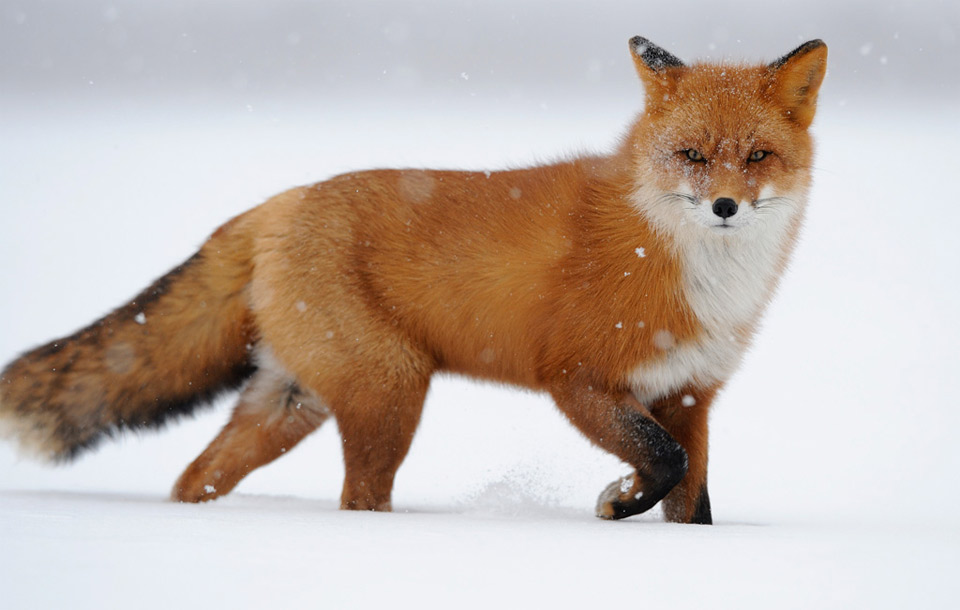
\includegraphics[height=2cm,width=2.5cm]{img/fox.jpg}} $\rightarrow \textrm{``fox''} \rightarrow [2.5, 4.7, 1.006, 0.75, ...]$
      \end{center}
    \end{frame}


    %%%%%%%%%%%%%%%%%%%%%%%%%%%%%%%%%%%%%%%%%%%%%%%%%%%%%%%%%%%%%%%%%%
    %%% Motivation
    \section{Motivation}
    \begin{frame}{\insertsection}
      \begin{example}
        \alt<1,4->{I\_{\tiny SRC} like\_{\tiny SNT} this\_{\tiny NON} car\_{\tiny TRG}}{0\_{\tiny SRC} 178\_{\tiny SNT} 35\_{\tiny NON} 56\_{\tiny TRG}}
      \end{example}

      \begin{example}
        \alt<1,4->{I\_{\tiny NON} drive\_{\tiny NON} this\_{\tiny NON} car\_{\tiny NON}}{0\_{\tiny NON} 208\_{\tiny NON} 35\_{\tiny NON} 56\_{\tiny NON}}
      \end{example}

      \only<3->{
      \begin{example}
        \only<3>{0\_{\tiny ???} 193\_{\tiny ???} 35\_{\tiny ???} 56\_{\tiny ???}}
        \only<4>{I\_{\tiny ???} love\_{\tiny ???} this\_{\tiny ???} car\_{\tiny ???}}
      \end{example}
}
    \end{frame}

    \begin{frame}{\insertsection}
      What would be the best way to represent words and their meanings?

      \begin{center}
        \begin{tikzpicture}
          [auto=right,scale=0.6,
            every node/.style={rectangle,draw=none,text width=2cm,font=\tiny,fill=none},
            word/.style={draw=none,fill=none}]

          \node[draw,align=center,text=white,fill=dodgerblue4] (string) at (6,6) {``fox''};

          \node(fox0) at (0,3) {a small wild animal that is related to
            dogs and that has a long pointed nose and a bushy tail};

          \node(fox0pic) at (0,0) {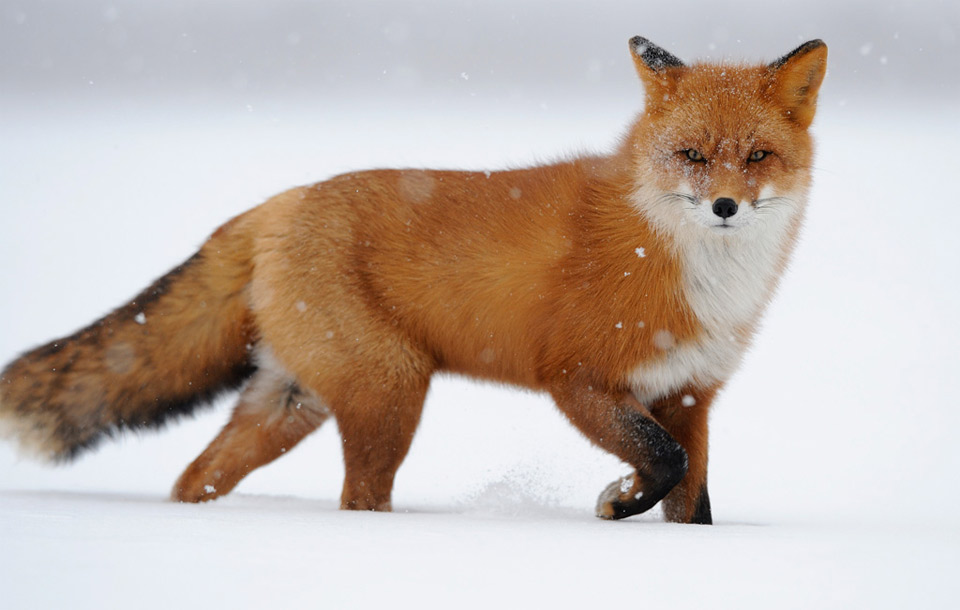
\includegraphics[height=1.5cm,width=2cm]{img/fox.jpg}};

          \node(fox1) at (4,3) {a clever crafty person};

          \node(fox1pic) at (4,0) {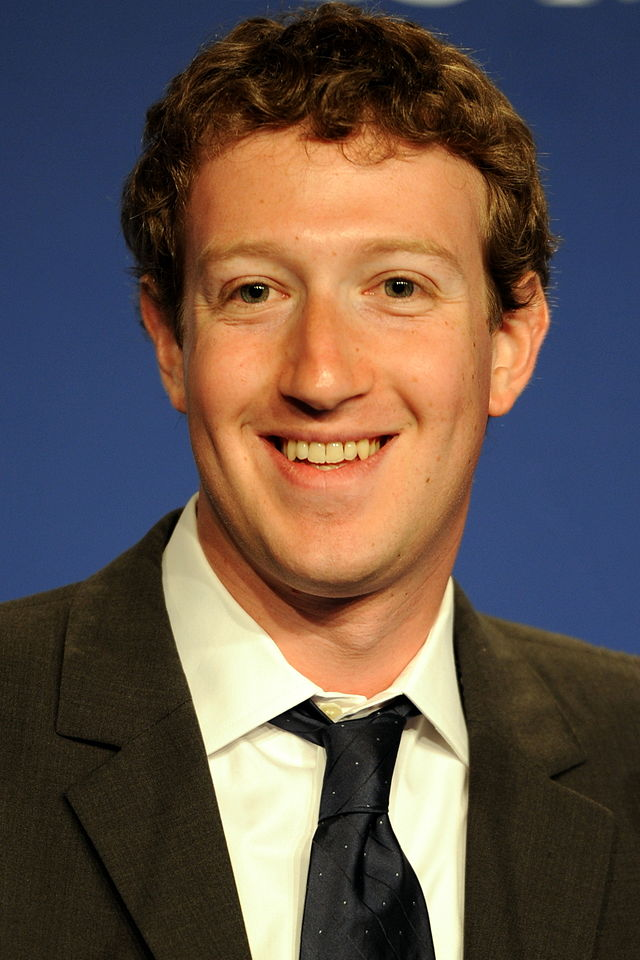
\includegraphics[height=2cm,width=1.5cm]{img/zuckerberg.jpg}};

          \node(fox2) at (8,3) {a good-looking young woman or man};

          \node(fox2pic) at (8,0) {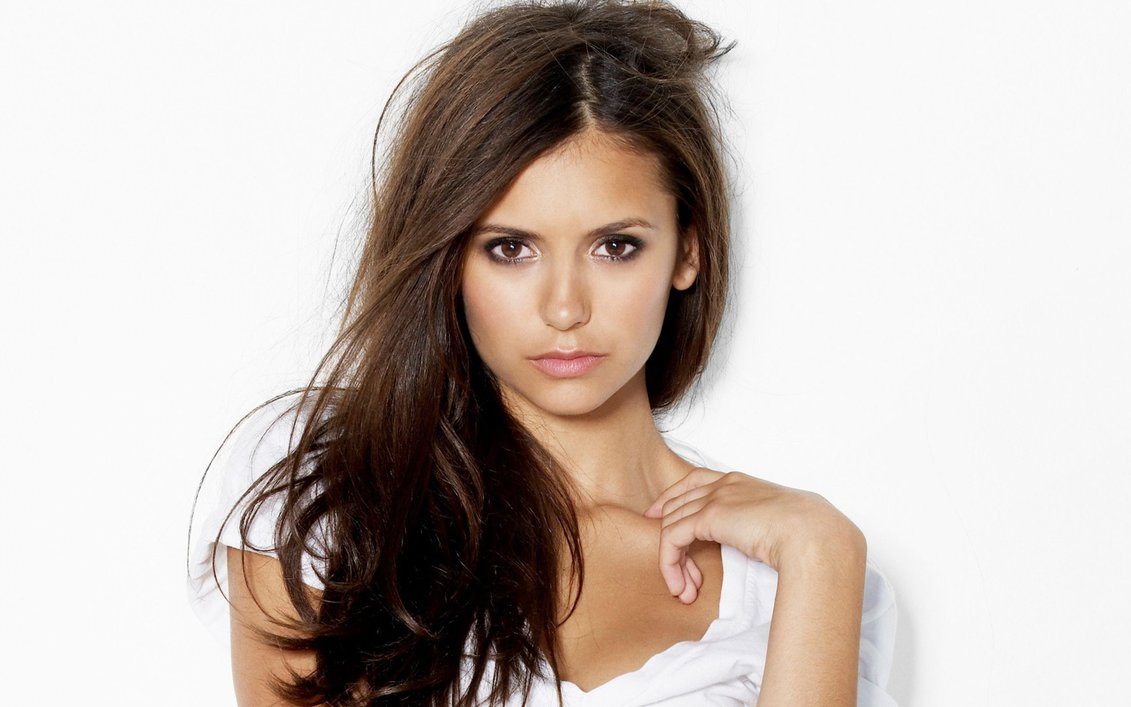
\includegraphics[height=1.5cm,width=1.8cm]{img/model.jpg}};

          \node(fox3) at (12,3) {a member of an American Indian people
            formerly living in what is now Wisconsin};

          \node(fox3pic) at (12,0) {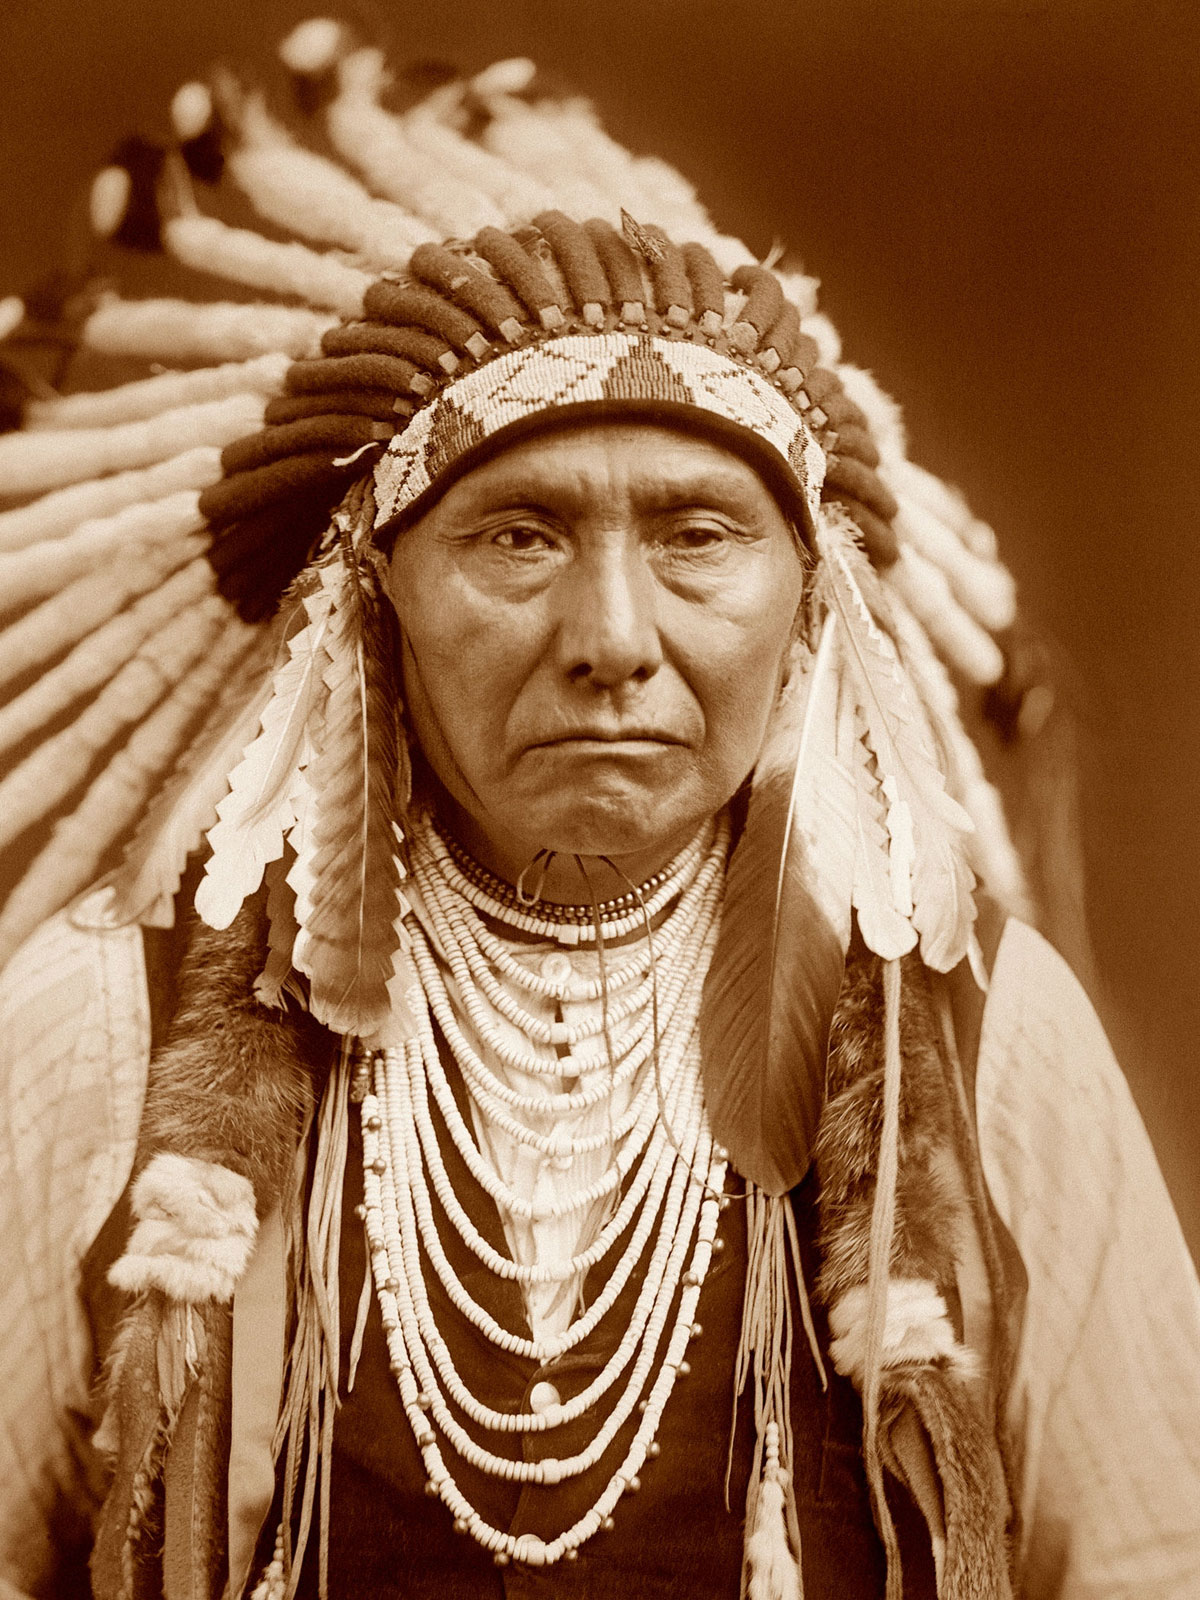
\includegraphics[height=2cm,width=1.5cm]{img/indian.jpg}};

          \foreach \from/\to in {string/fox0,string/fox1,string/fox2,string/fox3}
          \draw (\from) -- (\to);
        \end{tikzpicture}
      \end{center}
    \end{frame}

    \subsection{Model Change}
    \begin{frame}
      \frametitle{\insertsubsection}
      \tiny
      \vspace*{\fill}
      \begin{minipage}[t]{0.5\linewidth}
        \begin{center}
          \tikzset{mynode1/.style={}}
          \tikzset{mynode2/.style={}}
          \tikzset{mynode3/.style={}}
          \tikzset{mynode4/.style={}}
          \tikzset{mynode5/.style={}}
          \tikzset{mynode6/.style={}}
          \tikzset{mynode7/.style={}}
          \tikzset{mynode8/.style={}}
          \only<4->{\tikzset{mynode1/.style={text=white,fill=dodgerblue4}}}
          \only<5,9,11,12>{\tikzset{mynode2/.style={text=white,fill=dodgerblue4}}}
          \only<6,9,11>{\tikzset{mynode3/.style={text=white,fill=dodgerblue4}}}
          \only<7,9,11>{\tikzset{mynode4/.style={text=white,fill=dodgerblue4}}}
          \only<8,9,11>{\tikzset{mynode5/.style={text=white,fill=dodgerblue4}}}
          \only<10,11>{\tikzset{mynode6/.style={text=white,fill=dodgerblue4}}}
          \only<12>{\tikzset{mynode7/.style={text=white,fill=dodgerblue4}}}
          \only<10,11,12>{\tikzset{mynode8/.style={text=white,fill=dodgerblue4}}}

          \tikzset{myedge2/.style={color=white}}
          \tikzset{myedge3/.style={color=white}}
          \tikzset{myedge4/.style={color=white}}
          \tikzset{myedge5/.style={color=white}}
          \tikzset{myedge6/.style={color=white}}
          \tikzset{myedge7/.style={color=white}}
          \only<5,9,11,12>{\tikzset{myedge2/.style={color=black}}}
          \only<6,9,11>{\tikzset{myedge3/.style={color=black}}}
          \only<7,9,11>{\tikzset{myedge4/.style={color=black}}}
          \only<8,9,11>{\tikzset{myedge5/.style={color=black}}}
          \only<10,11>{\tikzset{myedge6/.style={color=black}}}
          \only<12>{\tikzset{myedge7/.style={color=black}}}

          \begin{tikzpicture}
            [auto=left,scale=0.6,
              every node/.style={rectangle,draw,font=\tiny,fill=gray84,minimum size=15pt},
              word/.style={draw=none,fill=none},
            ]

            \matrix (m) [matrix of math nodes,ampersand replacement=\&,fill=none,draw=none,rectangle,row sep=0.1cm,%
              column sep=0.8cm] {
              \node[mynode5]{SRC}; \& \node{SRC}; \& \node[mynode6]{SRC}; \& \node{SRC};\\
              \node[mynode4]{TRG}; \& \node{TRG}; \& \node[mynode6]{TRG}; \& \node{TRG};\\
              \node[mynode3]{STM}; \& \node[mynode1]{STM}; \& \node[mynode8]{STM}; \& \node[mynode7]{STM};\\
              \node[mynode2]{NON}; \& \node[mynode7]{NON}; \& \node[mynode8]{NON}; \& \node{NON};\\
              \node[word]{Ich}; \& \node[word]{mag}; \& \node[word]{diesen}; \& \node[word]{Politiker};\\
            };
            \draw[myedge2] (m-4-1) -- (m-3-2);
            \draw[myedge3] (m-3-1) -- (m-3-2);
            \draw[myedge4] (m-2-1) -- (m-3-2);
            \draw[myedge5] (m-1-1) -- (m-3-2);

            \draw[myedge6] (m-3-2) -- (m-4-3);
            \draw[myedge6] (m-3-2) -- (m-3-3);
            \draw[myedge6] (m-3-2) -- (m-2-3);
            \draw[myedge6] (m-3-2) -- (m-1-3);

            \draw[myedge7] (m-4-2) -- (m-3-3);
            \draw[myedge7] (m-4-3) -- (m-3-4);
          \end{tikzpicture}
        \end{center}
      \end{minipage}
      \begin{minipage}[t]{0.48\linewidth}
        \begin{center}
          \vspace*{\fill}
          \only<1>{
            \raggedright{\: Unnormalized probability of the tag sequence:}
            \begin{equation}
              \tilde{P}(X,Y) = exp\Big\{\sum_i{\Theta_{i} * f_{i}(x = X, y = Y)}\Big\}
            \end{equation}

            \raggedright{\: Normalized probability of the tag sequence:}
            \begin{equation}
              P(Y|X) = \frac{\tilde{P}(X,Y)}{\sum_{Y}\tilde{P}(X,Y)}
            \end{equation}
            \pause
          }

          \only<2>{
            \raggedright{\: Dataset:}
            \begin{equation*}
              \mathcal{D} = \{x[m],y[m]\}^M_{m=1}
            \end{equation*}

            \raggedright{\: Objective function:}
            \begin{equation}
              \begin{split}
              \Theta & = \argmax_{\Theta}(\prod_{m=1}^M{P(y[m]|x[m])})\\
              & = \argmax_{\Theta}(\sum_{m=1}^M{\ln(P(y[m]|x[m]))})
              \end{split}
            \end{equation}
            \pause
          }

          \only<3>{
            \raggedright{\: Partial derivative of the objective function:}
            \begin{equation}
              \begin{split}
              \frac{\partial \ell}{\partial \Theta_i} = & %
              \sum_{m=1}^M\sum_{t=1}^T{f_i(y^{(m)}_t, y^{(m)}_{t-1}, x^{(m)})} \\ %
              & - \sum_{m=1}^M\sum_{t=1}^T\sum_{y,y'}{f_i(y, y'|x^{(m)})} p(y,y'|x^{(m)})
              \end{split}
            \end{equation}
          }

          \only<11>{
            \raggedright{\: Marginals of state features:}
            \begin{equation*}
                m_s[t][i] = \frac{\alpha[t][i] * \beta[t][i]}{Z}
            \end{equation*}
          }
          \only<4,11>{
            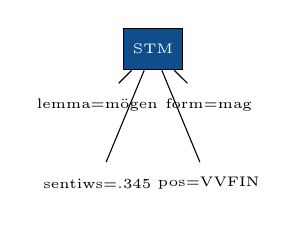
\begin{tikzpicture}
              [auto=right,scale=0.6,
                every node/.style={rectangle,draw=none,font=\tiny,fill=none,minimum size=15pt},
                word/.style={draw=none,fill=none}]
              \node[draw,align=center,text=white,fill=dodgerblue4] (n0) {STM};
              \node (n1) [below left of=n0] {lemma=m\"ogen};
              \node (n2) [below right of=n0] {form=mag};
              \node (n3) [below of=n1] {sentiws=.345};
              \node (n4) [below of=n2] {pos=VVFIN};
              \foreach \from/\to in {n1/n0,n2/n0,n3/n0,n4/n0}
              \draw (\from) -- (\to);
            \end{tikzpicture}
          }

          \only<5>{
            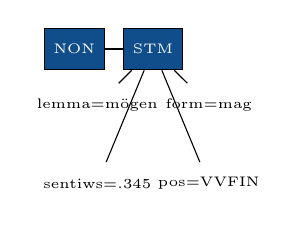
\begin{tikzpicture}
              [auto=right,scale=0.6,
                every node/.style={rectangle,draw=none,font=\tiny,fill=none,minimum size=15pt},
                word/.style={draw=none,fill=none}]
              \node[draw,align=center,text=white,fill=dodgerblue4] (n0) {STM};
              \node (n1) [below left of=n0] {lemma=m\"ogen};
              \node (n2) [below right of=n0] {form=mag};
              \node (n3) [below of=n1] {sentiws=.345};
              \node (n4) [below of=n2] {pos=VVFIN};
              \node (n5) [left of=n0,draw,text=white,fill=dodgerblue4] {NON};
              \foreach \from/\to in {n1/n0,n2/n0,n3/n0,n4/n0,n5/n0}
              \draw (\from) -- (\to);
            \end{tikzpicture}
          }

          \only<6>{
            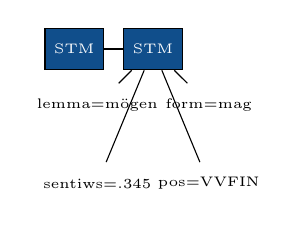
\begin{tikzpicture}
              [auto=right,scale=0.6,
                every node/.style={rectangle,draw=none,font=\tiny,fill=none,minimum size=15pt},
                word/.style={draw=none,fill=none}]
              \node[draw,align=center,text=white,fill=dodgerblue4] (n0) {STM};
              \node (n1) [below left of=n0] {lemma=m\"ogen};
              \node (n2) [below right of=n0] {form=mag};
              \node (n3) [below of=n1] {sentiws=.345};
              \node (n4) [below of=n2] {pos=VVFIN};
              \node (n5) [left of=n0,draw,text=white,fill=dodgerblue4] {STM};
              \foreach \from/\to in {n1/n0,n2/n0,n3/n0,n4/n0,n5/n0}
              \draw (\from) -- (\to);
            \end{tikzpicture}
          }

          \only<7>{
            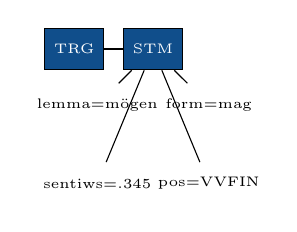
\begin{tikzpicture}
              [auto=right,scale=0.6,
                every node/.style={rectangle,draw=none,font=\tiny,fill=none,minimum size=15pt},
                word/.style={draw=none,fill=none}]
              \node[draw,align=center,text=white,fill=dodgerblue4] (n0) {STM};
              \node (n1) [below left of=n0] {lemma=m\"ogen};
              \node (n2) [below right of=n0] {form=mag};
              \node (n3) [below of=n1] {sentiws=.345};
              \node (n4) [below of=n2] {pos=VVFIN};
              \node (n5) [left of=n0,draw,text=white,fill=dodgerblue4] {TRG};
              \foreach \from/\to in {n1/n0,n2/n0,n3/n0,n4/n0,n5/n0}
              \draw (\from) -- (\to);
            \end{tikzpicture}
          }

          \only<8>{
            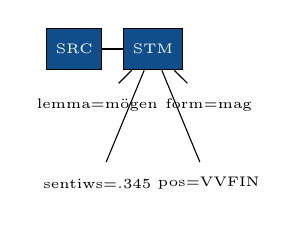
\begin{tikzpicture}
              [auto=right,scale=0.6,
                every node/.style={rectangle,draw=none,font=\tiny,fill=none,minimum size=15pt},
                word/.style={draw=none,fill=none}]
              \node[draw,align=center,text=white,fill=dodgerblue4] (n0) {STM};
              \node (n1) [below left of=n0] {lemma=m\"ogen};
              \node (n2) [below right of=n0] {form=mag};
              \node (n3) [below of=n1] {sentiws=.345};
              \node (n4) [below of=n2] {pos=VVFIN};
              \node (n5) [left of=n0,draw,text=white,fill=dodgerblue4] {SRC};
              \foreach \from/\to in {n1/n0,n2/n0,n3/n0,n4/n0,n5/n0}
              \draw (\from) -- (\to);
            \end{tikzpicture}
          }

          \only<9,10>{
            \raggedright{\: Computation of the alpha score:}
            \begin{equation*}
              \begin{split}
              \alpha[t][j] = \sum_i{\alpha[t-1][i] * \Theta_{i,j}} * state[t][j]
              \end{split}
            \end{equation*}
          }

          \only<10>{
            \raggedright{\: Computation of the beta score:}
            \begin{equation*}
              \begin{split}
              \beta[t][i] = & \sum_j{\beta[t+1][j] * \Theta_{i,j}}
              \end{split}
            \end{equation*}
          }

          \only<12>{
            \raggedright{\: Marginals of transition features:}
            \begin{equation*}
              \begin{split}
                m_t[i][j] = \sum_{t=1}^{T-1}\frac{\alpha[t][i] *
                  \Theta_{i,j} * \beta[t+1][j]  * state[t+1][j]}{Z}
              \end{split}
            \end{equation*}
          }
          \only<12>{
            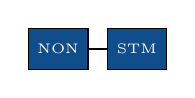
\begin{tikzpicture}
              [auto=center,
                every node/.style={rectangle,draw=none,font=\tiny,fill=none,minimum size=15pt},
                word/.style={draw=none,fill=none}]
              \node[draw,align=center,text=white,fill=dodgerblue4] (n0) {STM};
              \node (n1) [left of=n0,draw,text=white,fill=dodgerblue4] {NON};
              \draw (n0) -- (n1);
            \end{tikzpicture}
          }
        \end{center}
      \end{minipage}
      \vspace*{\fill}
    \end{frame}


    \begin{frame}
      \frametitle{\insertsubsection}
      \tiny
      \vspace*{\fill}
        \begin{center}
          \tikzset{mynode1/.style={}}
          \tikzset{mynode2/.style={}}
          \tikzset{mynode3/.style={}}
          \tikzset{mynode4/.style={}}
          \tikzset{mynode5/.style={}}
          \only<1->{\tikzset{mynode1/.style={text=white,fill=dodgerblue4}}}
          \only<1>{\tikzset{mynode2/.style={text=white,fill=dodgerblue4}}}
          \only<2->{\tikzset{mynode3/.style={text=white,fill=dodgerblue4}}}

          \tikzset{myedge1/.style={color=white}}
          \tikzset{myedge2/.style={color=white}}
          \tikzset{myedge3/.style={color=white}}
          \only<1>{\tikzset{myedge1/.style={color=black}}}
          \only<1->{\tikzset{myedge2/.style={color=black}}}
          \only<2->{\tikzset{myedge3/.style={color=black}}}

          \begin{tikzpicture}
            [auto=left,scale=0.6,
              every node/.style={rectangle,draw,font=\tiny,fill=gray84},
              word/.style={draw=none,fill=none},
            ]

            \matrix (m) [matrix of math nodes,ampersand replacement=\&,fill=none,draw=none,rectangle,row sep=0.8cm,%
              column sep=0.1cm] {
              \& \& \& \node[mynode3]{SRC}; \& \node[mynode3]{TRG}; \& \node[mynode1,label=below:{mag}]{STM}; \& \node[mynode3]{NON};%
              \& \& \& \\
              \node[mynode2,label=above:Ich]{SRC}; \& \node[mynode2]{TRG}; \& \node[mynode2]{STM}; \&
              \node[mynode2]{NON}; \& \& \& \node[mynode2]{SRC}; \& \node[mynode1]{TRG}; \& \node[mynode2]{STM}; \&
              \node[mynode2,label=above:Politiker]{NON}; \\
            };

            \draw[myedge1] (m-2-1) -- (m-1-6);
            \draw[myedge1] (m-2-2) -- (m-1-6);
            \draw[myedge1] (m-2-3) -- (m-1-6);
            \draw[myedge1] (m-2-4) -- (m-1-6);

            \draw[myedge1] (m-2-7) -- (m-1-6);
            \draw[myedge2] (m-2-8) -- (m-1-6);
            \draw[myedge1] (m-2-9) -- (m-1-6);
            \draw[myedge1] (m-2-10) -- (m-1-6);

            \draw[myedge3] (m-1-4) -- (m-2-8);
            \draw[myedge3] (m-1-5) -- (m-2-8);
            \draw[myedge3] (m-1-7) -- (m-2-8);
          \end{tikzpicture}

          \vspace*{\fill}
          \only<1,2>{
            \raggedright{\: Computation of the alpha score:}
            \begin{equation*}
              \alpha[p][j] = \prod_{c \in children}{\sum_i{\alpha[c][i] * \Theta_{i,j}}} * state[p][j]
            \end{equation*}
          }

          \only<2>{
            \raggedright{\: Computation of the beta score:}
            \begin{equation*}
              \beta[c][i] = \sum_j{\beta[p][j] * \Theta_{i,j} *
                \frac{\alpha[p][j]}{\sum_l{\alpha[c][l] * \Theta[l][j]}}}
            \end{equation*}
          }

          \only<3->{
            \raggedright{\: Marginals of state features:}
            \begin{equation*}
                m_s[t][i] = \frac{\alpha[t][i] * \beta[t][i]}{Z}
            \end{equation*}
          }

          \only<4>{
            \raggedright{\: Marginals of transition features:}
            \begin{equation*}
                m_s[t][i] = \frac{\alpha[c][i] * edge[i][j] * \beta[p][j] * \frac{\alpha[p][j]}{\alpha[c][l] * \Theta[l][j]}}{Z}
            \end{equation*}
          }
        \end{center}
      \vspace*{\fill}
    \end{frame}

    \begin{frame}
      \frametitle{\insertsubsection}
      Higher-order linear-chain CRF.
      \vspace*{\fill}
      \begin{center}
        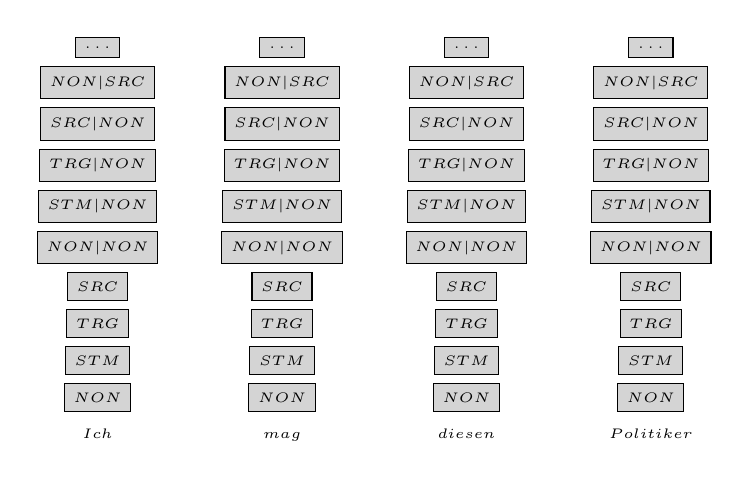
\begin{tikzpicture}
          [auto=left,scale=0.6,
            every node/.style={rectangle,draw,font=\tiny,fill=gray84},
            word/.style={draw=none,fill=none},
          ]

          \matrix (m) [matrix of math nodes,ampersand replacement=\&,fill=none,draw=none,rectangle,row sep=0.1cm,%
            column sep=0.8cm] {
            \node{\dots}; \& \node{\dots}; \& \node{\dots}; \& \node{\dots};\\
            \node{NON|SRC}; \& \node{NON|SRC}; \& \node{NON|SRC}; \& \node{NON|SRC};\\
            \node{SRC|NON}; \& \node{SRC|NON}; \& \node{SRC|NON}; \& \node{SRC|NON};\\
            \node{TRG|NON}; \& \node{TRG|NON}; \& \node{TRG|NON}; \& \node{TRG|NON};\\
            \node{STM|NON}; \& \node{STM|NON}; \& \node{STM|NON}; \& \node{STM|NON};\\
            \node{NON|NON}; \& \node{NON|NON}; \& \node{NON|NON}; \& \node{NON|NON};\\
            \node{SRC}; \& \node{SRC}; \& \node{SRC}; \& \node{SRC};\\
            \node{TRG}; \& \node{TRG}; \& \node{TRG}; \& \node{TRG};\\
            \node{STM}; \& \node{STM}; \& \node{STM}; \& \node{STM};\\
            \node{NON}; \& \node{NON}; \& \node{NON}; \& \node{NON};\\
            \node[word]{Ich}; \& \node[word]{mag}; \& \node[word]{diesen}; \& \node[word]{Politiker};\\
          };
        \end{tikzpicture}
      \end{center}
    \end{frame}

    \begin{frame}
      \frametitle{\insertsubsection}
      Higher-order semi-markov CRF \cite{Nguyen-14}.
      \vspace*{\fill}
      \begin{center}
        \tikzset{}
      \begin{tikzpicture}
          [auto=left,scale=0.6,
            every node/.style={rectangle,draw,font=\tiny,fill=gray84},
            word/.style={draw=none,fill=none},
            element2/.style={rectangle,top color=blue!20!white!20,bottom color=dodgerblue4,font=\tiny}
          ]

          \matrix (m) [matrix of math nodes,ampersand replacement=\&,fill=none,draw=none,rectangle,row sep=0.1cm,%
            column sep=0.8cm] {
            \node{\dots}; \& \node{\dots}; \& \node{\dots}; \& \node{\dots};\\
            \node{NON|SRC}; \& \node{NON|SRC}; \& \node{NON|SRC}; \& \node{NON|SRC};\\
            \node{SRC|NON}; \& \node{SRC|NON}; \& \node{SRC|NON}; \& \node{SRC|NON};\\
            \node{TRG|NON}; \& \node{TRG|NON}; \& \node{TRG|NON}; \& \node{TRG|NON};\\
            \node{STM|NON}; \& \node{STM|NON}; \& \node{STM|NON}; \& \node{STM|NON};\\
            \node{SRC}; \& \node{SRC}; \& \node{SRC}; \& \node{SRC};\\
            \node{TRG}; \& \node{TRG}; \& \node{TRG}; \& \node{TRG};\\
            \node{STM}; \& \node{STM}; \& \node{STM}; \& \node{STM};\\
            \node{NON}; \& \node{NON}; \& \node{NON}; \& \node{NON};\\
            \node[word]{Ich}; \& \node[word]{mag}; \& \node[word]{diesen}; \& \node[word]{Politiker};\\
          };
          \node[fit=(m-7-4)(m-7-4),element2,label={center:TRG}]{};
        \end{tikzpicture}
      \end{center}
    \end{frame}

    \begin{frame}
      \frametitle{\insertsubsection}
      Higher-order semi-markov CRF.
      \vspace*{\fill}
      \begin{center}
        \tikzset{}
      \begin{tikzpicture}
          [auto=left,scale=0.6,
            every node/.style={rectangle,draw,font=\tiny,fill=gray84},
            word/.style={draw=none,fill=none},
            element2/.style={rectangle,top color=blue!20!white!20,bottom color=dodgerblue4,font=\tiny}
          ]

          \matrix (m) [matrix of math nodes,ampersand replacement=\&,fill=none,draw=none,rectangle,row sep=0.1cm,%
            column sep=0.8cm] {
            \node{\dots}; \& \node{\dots}; \& \node{\dots}; \& \node{\dots};\\
            \node{NON|SRC}; \& \node{NON|SRC}; \& \node{NON|SRC}; \& \node{NON|SRC};\\
            \node{SRC|NON}; \& \node{SRC|NON}; \& \node{SRC|NON}; \& \node{SRC|NON};\\
            \node{TRG|NON}; \& \node{TRG|NON}; \& \node{TRG|NON}; \& \node{TRG|NON};\\
            \node{STM|NON}; \& \node{STM|NON}; \& \node{STM|NON}; \& \node{STM|NON};\\
            \node{SRC}; \& \node{SRC}; \& \node{SRC}; \& \node{SRC};\\
            \node{TRG}; \& \node{TRG}; \& \node{TRG}; \& \node{TRG};\\
            \node{STM}; \& \node{STM}; \& \node{STM}; \& \node{STM};\\
            \node{NON}; \& \node{NON}; \& \node{NON}; \& \node{NON};\\
            \node[word]{Ich}; \& \node[word]{mag}; \& \node[word]{diesen}; \& \node[word]{Politiker};\\
          };
          \node[fit=(m-7-3)(m-7-4),element2,label={center:TRG}]{};
        \end{tikzpicture}
      \end{center}
    \end{frame}

    \section*{Bibliography}
    \bibliography{bibliography}
    \bibliographystyle{plain}
    \end{document}
